\documentclass[a4paper,12pt]{article}
\usepackage[utf8]{inputenc}
\usepackage[spanish]{babel}
\usepackage{graphicx}
\usepackage{epstopdf}
\usepackage{graphicx}
\usepackage{listings}
\usepackage{array}
\usepackage{hyperref}
\usepackage[margin=25mm]{geometry}

\title{Documento de Requisitos}
\author{Carlos Bergen Dyck \and Gustav Svensk}
\begin{document}

\renewcommand{\arraystretch}{1.5}
\maketitle
\begin{center}
        {\large Versión 0.1}
\end{center}
\newpage


\section{Prefacio}
\begin{tabular}{p{3cm} p{12cm}}
        & Este es el Documento de Requisitos de “Air Guitar", un movimiento en donde se pretende tocar una guitarra. \\
        \textbf{Alcance del documento} & El Documento de Requisitos es la base
        de todo el desarrollo futuro de Nombre del Sistema. Describe los
        siguientes aspectos del sistema: propósito, contexto, requisitos
        funcionales, requisitos de pruebas, requisitos de calidad, requisitos
        de ambiente, arquitectura del sistema, requisitos del desarrollo,
        requisitos de post-desarrollo, y riesgos del proyecto. \\
        \textbf{Documentos relacionados} & Documento de Inicio de Proyecto,
        proyecto Nombre del Sistema, versión 1.1, 5/11/2013. \\
        \textbf{Autor} & Carlos Bergen Dyck y Gustav Svensk \\
        \textbf{Lectores} & Este documento está dirigido principalmente a los
        desarrolladores del proyecto, pero es de interés de todos los
        interesados en el mismo. \\
\end{tabular}

\section{Historia del Documento}
\begin{tabular}{|c|c|p{6cm}|p{4cm}|}
        \hline
        \textbf{Versión} & \textbf{Fecha} & \textbf{Explicación del cambio} &
        \textbf{Autor} \\ \hline
        0.1 & 30/10/2013 & Primer borrador & Carlos Bergen Dyck y Gustav Svensk \\
        \hline
\end{tabular}

\newpage
\tableofcontents

\listoftables

\listoffigures
\newpage

\section{Introducción}
En esta introducción se describe brevemente el contexto, objetivos y alcance
del proyecto a desarrollar, así como la documentación relativa al mismo. Esta
información está basada en el Documento de Inicio de Proyecto.

\subsection{Propósito}
Se generará un sonido de guitarra cuando un usuario esté simulando el tocar
una guitarra en el aire. El tono y el volumen se basarán en la posición de
las manos y la cadera del usuario.

\subsection{Alcance}
El sistema generará sonidos de acordes de guitarra. El tono se calculará en
base a la distancia entre la mano izquierda y la cadera. El volumen se
calculará en base a la velocidad de la mano derecha. Los sonidos se
reproducirán cuando la mano derecha pase sobre un área predefinida que
simulara el área de las cuerdas de una guitarra real. También sera posible cambiar el orden de las manos para poder adaptarse a zurdos. El sistema funcionará
con un solo usuario a la vez. Deberá estar parado, de frente al Kinect y a
una distancia de entre 0.8m  a 2.5m aproximadamente debido a las limitaciones
técnicas del Kinect \cite{depth_range}. Además debe existir una iluminación adecuada. Solo se
podrán tocar power chords (acordes que consisten de la nota fundamental, su
quinta y octavas). El rango de sonidos será similar a una guitarra real
siendo la nota fundamental más grave E1 y la más aguda E2, así cubriendo una
octava, generando un total de 12 acordes posibles en todos los semitonos. 

\subsection{Contexto}
“Air Guitar” es un movimiento en donde se pretende tocar una guitarra.
Usualmente estos movimientos carecen de sonido. Desde 1996 se ha realizado
anualmente el Campeonato Mundial de Air Guitar en Finlandia \cite{air_guitar}.

Kinect es un sensor de movimiento creado inicialmente para el Xbox 360.
Utiliza una cámara RGB y un sensor infrarrojo para detectar la distancia de
diferentes objetos y seguir los movimientos del cuerpo humano \cite{kinect_spec}.

Microsoft liberó el SDK de Kinect for Windows en el 2011 \cite{kinect_release}. Esto permitió a los
desarrolladores crear aplicaciones que usen el Kinect en C++/CLI, C\# y
Visual Basic .NET. Este SDK permite reconocer movimientos, gestos y comandos
de voz \cite{sdk}. La última version también incluye herramientas para quitar el fondo
para obtener un efecto de pantalla verde, mejoras para escanear y modelar
objetos 3D con Kinect Fusion y la opción para codificar en HTML5/JavaScript \cite{kinect_new}.

\section{Requisitos del Sistema}
Esta sección describe los requisitos funcionales del sistema, sus interfaces
externas, las condiciones de excepción y las clases de pruebas que se harán
para verificar que los requisitos se cumplen.
\subsection{Requisitos Funcionales}
Los requisitos funcionales definen el comportamiento del sistema. Es decir,
describen lo que debe hacer el sistema.
\begin{table}[h!]
        \centering
        \begin{tabular}{c l}
                \textbf{RF1} & Obtener la posición de las manos y la cadera \\
                \textbf{RF2} & Obtener la velocidad de la mano derecha \\
                \textbf{RF3} & Calcular tono y volumen en base a la posición
                y velocidad de las manos \\
                \textbf{RF4} & Reproducir sonido en base al tono y volumen \\
                \textbf{RF5} & Proyectar modelo 3D de guitarra \\
        \end{tabular}
        \caption{Requisitos funcionales}
        \label{tab:req_func}
\end{table}

\subsection{Requisitos de Interfaces}
La tabla~\ref{tab:event} muestra la lista de eventos externos a los que el sistema responde.
La primera columna es el nombre del evento; la segunda es la descripción del
mismo. El “iniciador” es la componente externa al sistema que inicia el evento.
Los parámetros son los datos asociados al evento. La respuesta es el nombre de
una respuesta, cuya descripción está en la tabla~\ref{tab:respuesta}.
La tabla~\ref{tab:respuesta} muestra las respuestas del sistema frente a eventos externos.
\begin{table}[hb]
        \centering
        \begin{tabular}{|p{2cm}|p{4cm}|c|p{3cm}|p{25mm}|}
                \hline
                \textbf{Evento} & \textbf{Descripción} & \textbf{Iniciador} &
                \textbf{Parámetros} & \textbf{Respuesta} \\
                \hline
                Recepción de datos de Kinect & Se recibe información del
                Kinect sobre los puntos del esqueleto. & Kinect & Colección
                de puntos 3D del esqueleto del usuario. & Tono y volumen \\
                \hline
                Tocar guitarra & Se reproduce un sonido de guitarra cuando la
                mano entra a un área de reproducción. & Usuario & Velocidad de
                la mano derecha y posición de la mano izquierda & Reproducción
                de sonido \\
                \hline
                Proyectar guitarra & Se proyecta un modelo 3D de una guitarra sobre la imagen del usuario. \\
                \hline
        \end{tabular}
        \caption{Eventos externos}
        \label{tab:event}
\end{table}

\begin{table}[h!]
        \centering
        \begin{tabular}{|p{3cm}|p{6cm}|p{4cm}|}
                \hline
                \textbf{Respuesta} & \textbf{Descripción} & \textbf{Parámetros} \\
                \hline
                Tono y volumen & Calcula el tono basado en la distancia entre
                los puntos de la mano izquierda y la cadera.
                Si la mano izquierda esta muy lejos de la cadera simplemente toca la nota mas grave, igual cuando este muy cerca simplemente toca la nota mas aguda. Calcula el volumen
                basado en la velocidad de la mano derecha al entrar a un area predefinida. Existira un volumen máximo. & Colección de
                puntos 3D del esqueleto del usuario. \\
                \hline
                Reproducción de sonido & Reproduce el sonido correspondiente al
                tono en el que se encuentra el sistema a un volumen basado en
                la velocidad de la mano derecha. Se podran escoger entre diferentes tipos de sonidos pregrabados, por ejemplo guitarra eléctrica o acustica. & Velocidad de mano derecha. \\
                \hline
        \end{tabular}
        \caption{Respuestas del sistema}
        \label{tab:respuesta}
\end{table}

\newpage
\section{Requisitos de Ambiente}
Esta sección describe el hardware y software relevante para el sistema Air
Guitar.
\subsection{Requisitos del Ambiente de Desarrollo}
\subsubsection{Hardware de Desarrollo}
\label{subsubsec:hardware}

\begin{itemize}
        \item Kinect para Windows, utilizado para obtener las posiciones de las
                manos y el cuerpo del usuario.
        \item Windows 7, Windows 8, Windows Embedded Standard 7, o Windows
                Embedded POSReady 7.
        \item Procesador 32 bit (x86) o 64 bit (x64) 
        \item Procesador Dual-core 2.66-GHz o más rápido. 
        \item Bus USB 2.0 dedicado
        \item 2 GB RAM
\end{itemize}

\subsubsection{Software de Desarrollo}
\label{subsubsec:software}

\begin{itemize}
	\item Se programara en el lenguaje C++ con Visual Studio.
	\item Se utilizara el SDK 1.8 de Kinect for Windows para la comunicación con entre el dispositivo Kinect y la aplicación. 
	\item Se utilizara OpenFrameworks para la reproducción del audio y la proyección de la guitarra.
\end{itemize}

\section{Arquitectura del Sistema}

\subsection{Diagrama de Flujo de Datos}

La figura~\ref{fig:flujo} muestra los flujos de datos en el sistema.

\begin{figure}[h!]
        \centering
        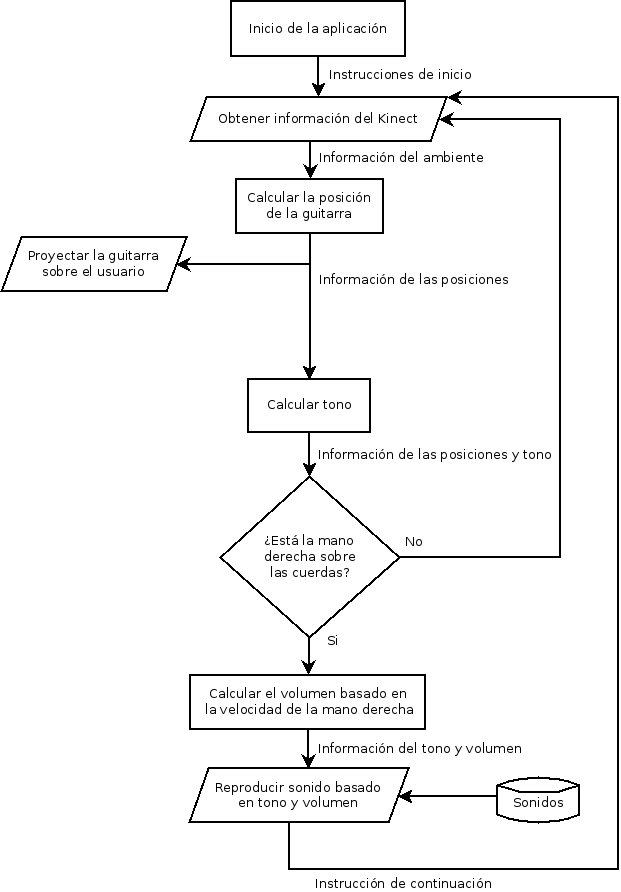
\includegraphics[width=0.6\textwidth]{../imagenes/diagrama_de_flujo.png}
        \caption{Diagrama de flujo de datos}
        \label{fig:flujo}
\end{figure}
\newpage

\subsection{Descripción de Módulos}
\subsubsection{Obtener información del Kinect(IK)}
Se obtiene la posición de los puntos del esqueleto del usuario entregados por el
Kinect.
\subsubsection{Calcular la posición de la guitarra(CG)}
Con los puntos obtenidos del Kinect se calcula la posición de la guitarra con la
posición de la cadera y de la mano izquierda.
\subsection{Proyectar la guitarra sobre el usuario(PG)}
Se proyecta un modelo 3D de la guitarra basado en la posición obtenida de la
cadera y la mano izquierda.
\subsubsection{Calcular tono(CT)}
Se calculará el tono basado en la distancia entre la cadera y la mano izquierda.
\subsubsection{¿Está la mano derecha sobre las cuerdas?(MD)}
Se verá si la mano derecha se encuentra sobre un área predefinida alrededor del
punto de la cadera que simulara el área de las cuerdas de una guitarra real.
\subsubsection{Calcular el volumen(CV)}
Se calculará el volumen basado en la velocidad de la mano derecha.
\subsubsection{Reproducir sonido(RS)}
Se reproducirá el sonido correspondiente al tono calculado al volumen
previamente calculado.
\subsubsection{Sonidos(SO)}
Una colección de sonidos de acordes de guitarra grabados previamente.
\subsection{Matriz de Requisitos Funcionales y Componentes}
\begin{table}[h!]
        \centering
        \begin{tabular}{|c|c|c|c|c|c|c|c|c|}
                \hline
                 & \textbf{IK} & \textbf{CG} & \textbf{PG} & \textbf{CT} &
                 \textbf{MD} & \textbf{CV} & \textbf{RS} & \textbf{SO} \\
                \hline
                \textbf{RF1} & X & & & & & & & \\
                \hline
                \textbf{RF2} & X & & & & & & & \\
                \hline
                \textbf{RF3} & & & & X & & X & & \\
                \hline
                \textbf{RF4} & & & & & X & & X & X \\
                \hline
                \textbf{RF5} & & X & X & & & & & \\
                \hline
        \end{tabular}
        \caption{Matriz de requisitos funcionales y componentes}
        \label{tab:matrizrequisitos}
\end{table}

\section{Gestión de Riesgos}
\subsection{Supuestos}
\begin{itemize}
        \item La precisión y el tiempo de respuesta del Kinect será suficiente
                para dar una experiencia similar a una guitarra real
        \item La iluminación donde se instala el sistema será en el rango donde
                funciona el Kinect
\end{itemize}

\subsection{Dependencias}
\begin{itemize}
        \item Disponibilidad de un Kinect for Windows
        \item Un lugar con buena iluminación y suficiente espacio para moverse.
\end{itemize}

\subsection{Restricciones}
\begin{itemize}
        \item Hardware necesario según~\ref{subsubsec:hardware}
        \item Software necesario según~\ref{subsubsec:software}
\end{itemize}

\subsection{Riesgos}
A continuación se indican los principales riesgos del proyecto.
\subsubsection{Disponibilidad de un Kinect}
Intentamos a planear los tiempos cuando necesitamos un Kinect para reservarlo.
También intentamos avanzar el proyecto en áreas que no dependen del Kinect.
\subsubsection{Precisión de Kinect no suficiente}
Si la precisión y tiempo de respuesta del Kinect no son suficientes podemos
expandir la zona de reproducción del sonido.
\subsubsection{El procesamiento tarda demasiado}
Si el procesamiento para los cálculos de tono y volumen tarda demasiado tiempo
buscamos algoritmos mas rápidos o usamos un volumen constante.
\subsubsection{Intentar hacer Stagedive}
Si se tiene ganas de hacer Stagedive recomendamos tener una audiencia o colchón
presente.
\subsubsection{Falta de tiempo para el proyecto}
Si falta tiempo para el proyecto no hacemos la proyección de la guitarra.

\newpage 
\appendix 
\newpage

\addcontentsline{toc}{section}{Referencias}
\begin{thebibliography}{99}
\bibitem{depth_range}\url{http://msdn.microsoft.com/en-us/library/hh973078.aspx#Depth_Ranges} \\
        Microsoft Developer Network, 05 Nov 2013
\bibitem{air_guitar}\url{https://en.wikipedia.org/wiki/Air_guitar#Contests} \\
        Wikipedia, 05 Nov 2013
\bibitem{kinect_spec}\url{http://msdn.microsoft.com/en-us/library/jj131033.aspx} \\
        Microsoft Developer Network, 05 Nov 2013
\bibitem{kinect_release}\url{http://en.wikipedia.org/wiki/Kinect#History} \\
        Wikipedia, 05 Nov 2013
\bibitem{sdk}\url{http://msdn.microsoft.com/en-us/library/hh855347.aspx} \\
        Microsoft Developer Network, 05 Nov 2013
\bibitem{kinect_new}\url{http://blogs.msdn.com/b/kinectforwindows/archive/2013/09/16/updated-sdk-with-html5-kinect-fusion-improvements-and-more.aspx} \\
        Kinect for Windows Blog, 05 Noc 2013
\end{thebibliography}

\end{document} 
%%% Local Variables: %%% mode: latex %%% TeX-master: t %%% End:
